\documentclass{standalone}
\usepackage{tikz}
\usetikzlibrary{patterns, positioning}
\usepackage[sfdefault]{ClearSans} %% option 'sfdefault' activates Clear Sans as the default text font
\usepackage[T1]{fontenc}

\begin{document}
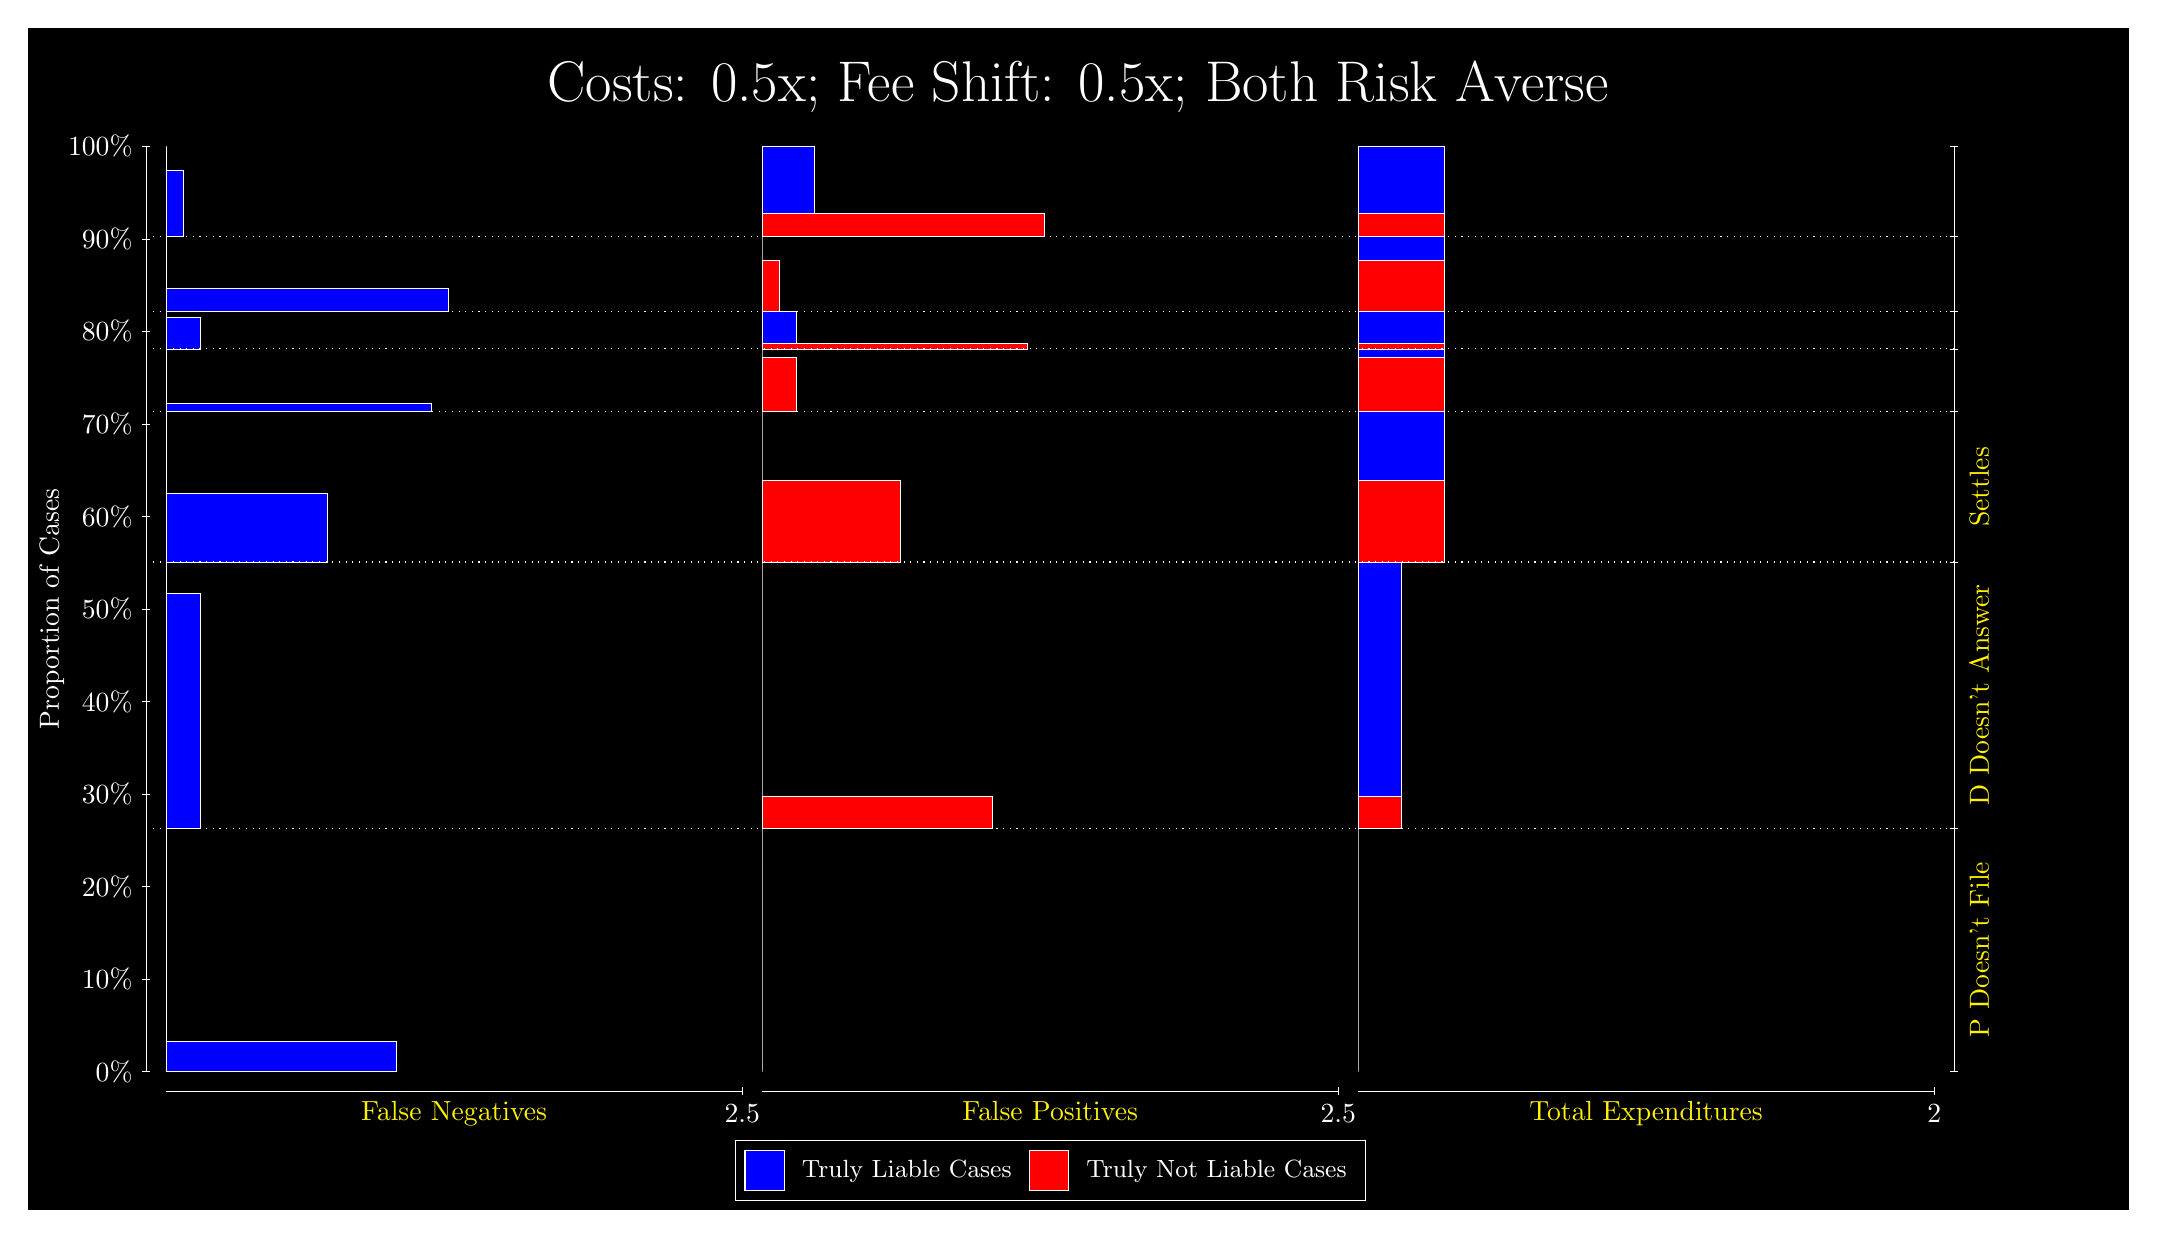
\begin{tikzpicture}
\draw[fill=black] (0,0) rectangle (26.667,15);
\draw[text=white] (0,13.5) rectangle (26.667,15) node[midway] {\huge Costs: 0.5x; Fee Shift: 0.5x; Both Risk Averse};
\draw[white, very thin] (1.5,1.75) -- (1.5,13.5);
\node[rotate=90, text=white, anchor=center] at (0.3, 7.625) {Proportion of Cases};
\draw[white, very thin] (1.45,1.75) -- (1.55,1.75);
\node[text=white, anchor=east] at (1.45, 1.75) {0\%};
\draw[white, very thin] (1.45,2.925) -- (1.55,2.925);
\node[text=white, anchor=east] at (1.45, 2.925) {10\%};
\draw[white, very thin] (1.45,4.1) -- (1.55,4.1);
\node[text=white, anchor=east] at (1.45, 4.1) {20\%};
\draw[white, very thin] (1.45,5.275) -- (1.55,5.275);
\node[text=white, anchor=east] at (1.45, 5.275) {30\%};
\draw[white, very thin] (1.45,6.45) -- (1.55,6.45);
\node[text=white, anchor=east] at (1.45, 6.45) {40\%};
\draw[white, very thin] (1.45,7.625) -- (1.55,7.625);
\node[text=white, anchor=east] at (1.45, 7.625) {50\%};
\draw[white, very thin] (1.45,8.8) -- (1.55,8.8);
\node[text=white, anchor=east] at (1.45, 8.8) {60\%};
\draw[white, very thin] (1.45,9.975) -- (1.55,9.975);
\node[text=white, anchor=east] at (1.45, 9.975) {70\%};
\draw[white, very thin] (1.45,11.15) -- (1.55,11.15);
\node[text=white, anchor=east] at (1.45, 11.15) {80\%};
\draw[white, very thin] (1.45,12.325) -- (1.55,12.325);
\node[text=white, anchor=east] at (1.45, 12.325) {90\%};
\draw[white, very thin] (1.45,13.5) -- (1.55,13.5);
\node[text=white, anchor=east] at (1.45, 13.5) {100\%};

\draw[white, very thin] (24.457,1.75) -- (24.457,13.5);
\draw[white, very thin] (24.407,1.75) -- (24.507,1.75);
\node[anchor=west] at (24.407, 1.75) {};
\draw[white, very thin] (24.407,4.8405) -- (24.507,4.8405);
\node[anchor=west] at (24.407, 4.8405) {};
\draw[white, very thin] (24.407,8.2215) -- (24.507,8.2215);
\node[anchor=west] at (24.407, 8.2215) {};
\draw[white, very thin] (24.407,10.129) -- (24.507,10.129);
\node[anchor=west] at (24.407, 10.129) {};
\draw[white, very thin] (24.407,10.927) -- (24.507,10.927);
\node[anchor=west] at (24.407, 10.927) {};
\draw[white, very thin] (24.407,11.403) -- (24.507,11.403);
\node[anchor=west] at (24.407, 11.403) {};
\draw[white, very thin] (24.407,12.355) -- (24.507,12.355);
\node[anchor=west] at (24.407, 12.355) {};
\draw[white, very thin] (24.407,13.5) -- (24.507,13.5);
\node[anchor=west] at (24.407, 13.5) {};

\draw[white, very thin, fill=blue] (1.75,1.75) rectangle (4.6775,2.1292);
\draw[white, very thin, fill=red] (1.75,2.1292) rectangle (1.75,4.8405);
\draw[white, very thin, fill=blue] (1.75,4.8405) rectangle (2.1891,7.8189);
\draw[white, very thin, fill=red] (1.75,7.8189) rectangle (1.75,8.2215);
\draw[white, very thin, fill=blue] (1.75,8.2215) rectangle (3.7993,9.0879);
\draw[white, very thin, fill=red] (1.75,9.0879) rectangle (1.75,10.129);
\draw[white, very thin, fill=blue] (1.75,10.129) rectangle (5.1167,10.233);
\draw[white, very thin, fill=red] (1.75,10.233) rectangle (1.75,10.927);
\draw[white, very thin, fill=blue] (1.75,10.927) rectangle (2.1891,11.329);
\draw[white, very thin, fill=red] (1.75,11.329) rectangle (1.75,11.403);
\draw[white, very thin, fill=blue] (1.75,11.403) rectangle (5.3362,11.702);
\draw[white, very thin, fill=red] (1.75,11.702) rectangle (1.75,12.355);
\draw[white, very thin, fill=blue] (1.75,12.355) rectangle (1.9696,13.201);
\draw[white, very thin, fill=red] (1.75,13.201) rectangle (1.75,13.5);
\draw[white, very thin, fill=red] (9.3189,1.75) rectangle (9.3189,4.4613);
\draw[white, very thin, fill=blue] (9.3189,4.4613) rectangle (9.3189,4.8405);
\draw[white, very thin, fill=red] (9.3189,4.8405) rectangle (12.246,5.2431);
\draw[white, very thin, fill=blue] (9.3189,5.2431) rectangle (9.3189,8.2215);
\draw[white, very thin, fill=red] (9.3189,8.2215) rectangle (11.075,9.2623);
\draw[white, very thin, fill=blue] (9.3189,9.2623) rectangle (9.3189,10.129);
\draw[white, very thin, fill=red] (9.3189,10.129) rectangle (9.758,10.823);
\draw[white, very thin, fill=blue] (9.3189,10.823) rectangle (9.3189,10.927);
\draw[white, very thin, fill=red] (9.3189,10.927) rectangle (12.686,11.001);
\draw[white, very thin, fill=blue] (9.3189,11.001) rectangle (9.758,11.403);
\draw[white, very thin, fill=red] (9.3189,11.403) rectangle (9.5384,12.056);
\draw[white, very thin, fill=blue] (9.3189,12.056) rectangle (9.3189,12.355);
\draw[white, very thin, fill=red] (9.3189,12.355) rectangle (12.905,12.654);
\draw[white, very thin, fill=blue] (9.3189,12.654) rectangle (9.9776,13.5);
\draw[white, very thin, fill=red] (16.888,1.75) rectangle (16.888,4.4613);
\draw[white, very thin, fill=blue] (16.888,4.4613) rectangle (16.888,4.8405);
\draw[white, very thin, fill=red] (16.888,4.8405) rectangle (17.437,5.2431);
\draw[white, very thin, fill=blue] (16.888,5.2431) rectangle (17.437,8.2215);
\draw[white, very thin, fill=red] (16.888,8.2215) rectangle (17.986,9.2623);
\draw[white, very thin, fill=blue] (16.888,9.2623) rectangle (17.986,10.129);
\draw[white, very thin, fill=red] (16.888,10.129) rectangle (17.986,10.823);
\draw[white, very thin, fill=blue] (16.888,10.823) rectangle (17.986,10.927);
\draw[white, very thin, fill=red] (16.888,10.927) rectangle (17.986,11.001);
\draw[white, very thin, fill=blue] (16.888,11.001) rectangle (17.986,11.403);
\draw[white, very thin, fill=red] (16.888,11.403) rectangle (17.986,12.056);
\draw[white, very thin, fill=blue] (16.888,12.056) rectangle (17.986,12.355);
\draw[white, very thin, fill=red] (16.888,12.355) rectangle (17.986,12.654);
\draw[white, very thin, fill=blue] (16.888,12.654) rectangle (17.986,13.5);
\draw[white, dotted] (1.5,4.8405) -- (24.457,4.8405);
\draw[white, dotted] (1.5,8.2215) -- (24.457,8.2215);
\draw[white, dotted] (1.5,10.129) -- (24.457,10.129);
\draw[white, dotted] (1.5,10.927) -- (24.457,10.927);
\draw[white, dotted] (1.5,11.403) -- (24.457,11.403);
\draw[white, dotted] (1.5,12.355) -- (24.457,12.355);
\draw[white, very thin] (1.75,1.5) -- (9.0689,1.5);
\node[text=yellow, anchor=north] at (5.4094, 1.5) {False Negatives};
\draw[white, very thin] (9.0689,1.45) -- (9.0689,1.55);
\node[text=white, anchor=north] at (9.0689, 1.45) {2.5};

\draw[white, very thin] (9.3189,1.5) -- (16.638,1.5);
\node[text=yellow, anchor=north] at (12.978, 1.5) {False Positives};
\draw[white, very thin] (16.638,1.45) -- (16.638,1.55);
\node[text=white, anchor=north] at (16.638, 1.45) {2.5};

\draw[white, very thin] (16.888,1.5) -- (24.207,1.5);
\node[text=yellow, anchor=north] at (20.547, 1.5) {Total Expenditures};
\draw[white, very thin] (24.207,1.45) -- (24.207,1.55);
\node[text=white, anchor=north] at (24.207, 1.45) {2};

\node[text=yellow, centered, rotate=90] at (24.777, 3.2953) {P Doesn't File};
\node[text=yellow, centered, rotate=90] at (24.777, 6.531) {D Doesn't Answer};
\node[text=yellow, centered, rotate=90] at (24.777, 9.1751) {Settles};





\draw (12.978300999999998,1.5) node[draw=none] (baseCoordinate) {};
\begin{scope}[align=center]
        \matrix[scale=0.5, draw=white, below=0.5cm of baseCoordinate, nodes={draw}, column sep=0.1cm]{
            \node[rectangle, draw, minimum width=0.5cm, minimum height=0.5cm, fill=blue] {}; &
            \node[draw=none, font=\small, text=white] (B) {Truly Liable Cases}; &
            \node[rectangle, draw, minimum width=0.5cm, minimum height=0.5cm, fill=red] {}; &
            \node[draw=none, font=\small, text=white] (B) {Truly Not Liable Cases}; \\
            };
\end{scope}

\end{tikzpicture}
\end{document}